\documentclass[11pt,a4paper,english]{article}
\usepackage{natbib}  % Adds support for different citation styles
\bibliographystyle{chicago}
\usepackage[T1]{fontenc}
\usepackage[utf8]{inputenc}
\usepackage{babel}
\usepackage{blindtext}
\usepackage[nodayofweek,level]{datetime}
\newdate{date}{03}{12}{2024}
\date{\displaydate{date}}
\usepackage[a4paper,margin=1in]{geometry}
\usepackage{graphicx}
\usepackage{setspace}
\usepackage{amsmath}
\usepackage{hyperref}
\usepackage{tabularx}
\usepackage{booktabs}
\doublespacing



\title{A Methodology for Measuring Market Inefficiency, and Its Relationship to the Value Spread 
\thanks{Code and data supporting this analysis is available at: \url{https://github.com/Aman-Rana-02/Irrational_Value_Spreads}}}
\author{%
  Aman Rana\\
  % \small Department of Computer Science\\
  % \small University of Toronto\\
  % \small\texttt{aman.rana@mail.utoronto.ca}
}

\begin{document}
  \maketitle

  \begin{abstract}
    \noindent Extending the work of \citet{boguth_2023}, we propose a method to measure the level of market inefficiency using unbiasedness regressions and the S\&P500 index.
    We find that the market is not uniformly efficient and goes through periods of higher inefficiency reverting to efficiency. We find that the value spread—the ratio of the average book-to-market of expensive stocks to that of cheap stocks—is correlated with market inefficiency. 
    By demonstrating that wider value spreads comove with our measure of market inefficiency, we can empirically support \citet{asness_2024}'s intuition 
    that high spreads during events such as the dot-com bubble and COVID-19 could reflect mispricing rather than fundamental changes in the notion of value. 
    This evidence strengthens the case that the value premium is still alive but has been masked by market inefficiency. 
    This has implications for risk-premia based strategies and portfolio management.
  \end{abstract}

  \newpage
  \tableofcontents

  \newpage
  \section{Introduction}
% A comment on market efficiency.
% - Why is efficiency important
% - What is Value? What is its relation to market efficiency?
% A comment on current scoring systems of market efficiency.
% A comment on Boguth paper's method
% We apply the $Beta\_SSE$ score and find:
% - The market is not uniformly efficient
% - The market goes through periods of inefficiency and reverts to efficiency.
% - The market has been increasingly inefficient in the last decade. 
% - The market inefficiency is cointegrated with the value spread.

% \citet{fama_random_walk}'s efficient market hypothesis is the prevailing model of the market.
%  Simply, in its strongest form, stock prices reflect all available information, public and private. In practice, the market is believed 
%  to be semi-strong efficient, where prices reflect all public information. Market efficiency is generally tested by testing the random-walk 
%  nature of stock prices (\cite{fama_random_walk} \cite{lim_brooks_2010}). The efficiency of a market is important because of its relation to 
%  the compensation of risk. Investors should be compensated for taking on systematic risk, but only in an efficient market. 
%  An example is the classical Value risk factor from \cite{fama_french_1993}, which argues investors are compensated for holding firms 
%  with a higher book-to-market ratio, reflecting the higher risks associated with undervalued or distressed companies.
%  \citet{asness_2024} argues that the market has become less efficient, and uses the value spread as a proxy for market efficiency to show this, where the
%  value spread is the ratio of expensive to cheap stock valuations. He shows that value spreads have been increasing for the last decade, and uses this as evidence that the market is less efficient.
% This conclusion relies on the assumption that abnormally high value spreads are detached from fundamentals, which he argues is the case, pointing at \citet{maloney_moskowitz_2020}
% and other works, which are not able to robustly explain the high value spreads. A proof by contradiction.

% We are able to independently show a timeseries of the level of market efficiency, and then show its relationship with the value spread.
% We arrive at the same conclusion, however, from a market efficiency first approach.

% \citet{boguth_2023} uses unbiasedness regressions to show the efficiency of the market around events. We first use a similar method
% to show the market is generally efficient across a 3 year window. We then construct a score, called \textbf{$Beta\_SSE$},
% which measures the level of market efficiency at a point-in-time by using a plot of the Betas from these unbiasedness regressions.
% By taking a rolling window of unbiasedness regressions, we get a timeseries of the relative level of market efficiency. 
% We find that the market is not uniformly efficient, and goes through periods of higher inefficiency reverting to efficiency. 
% We also find that the market has been increasingly inefficient in the last decade. We compare the timeseries of market inefficiency 
% to the timeseries of the value spread, and find that they are cointegrated.

\indent \citet{fama_random_walk}'s efficient market hypothesis posits that markets incorportate all information rationally and instantaneously. While 
this is an extreme assumption, it is established that markets tend to some form of efficiency. %\textbf{DO I NEED TO FIND PAPERS FOR THIS?}
In an efficient market, investors are compensated for taking on systematic risk, therefore, understanding the level of 
market efficiency can be used to asses whether market participants will be rewarded fairly for the risks they bear.

"Value" in classical factor investing refers to stocks with high book-to-market ratios as per \citet{fama_french_1993}, typically considered undervalued or distressed. 
Its relationship with market efficiency is critical: if markets are efficient, an investor should be rewarded for holding a portfolio of under-valued stocks. 
However, when inefficiencies arise, value stocks may become mispriced, with the market willing to pay more for already 'expensive' stocks, and
less for already 'cheap' stocks. In these periods, investors may consider that the definition of value has changed, the subjective measure of 
'expensive' and 'cheap' has shifted. We can define a value spread as the ratio of the value of expensive stocks to the value of cheap stocks.
In this paper we show that generally, periods of inflated value spreads are correlated with increasing inefficiency,
therefore we suggest that abnormal value spreads are not reflective of a fundamental change in the market, but rather a mispricing.

Existing methods for measuring market efficiency typically focus on testing whether stock prices follow a random walk
(\cite{fama_random_walk}, \cite{lim_brooks_2010}). However, these methods often fail to capture variations in the level of efficiency over time.
A more dynamic approach is needed to reflect the market’s changing behavior.

\citet{boguth_2023} uses unbiasedness regressions to examine price informativeness around FOMC meetings. 
This method visually shows us how prices adjust to information flow, in speed, and under or overreaction, using $R^2$s and $\beta$s over the unbiasedness regression window,
which is useful in an approach for measuring efficiency.

Building on this, we introduce the \textit{$Beta\_SSE$} score, which measures market efficiency at a point in time. 
By applying unbiasedness regressions within a rolling window, and constructing the \textit{$Beta\_SSE$} representation, we create a time series that tracks the level of market 
efficiency. \newline
\newline
Our findings show that:
\begin{itemize}
    \item The market is not uniformly efficient. Instead, it experiences cycles of inefficiency followed by reversion to efficiency.
    \item Over the last decade, inefficiency has been increasing, suggesting that the market has become less adept at incorporating available information into prices on longer time-scales.
    \item Furthermore, this rising inefficiency is cointegrated with the value spread, indicating a strong link between the weakness of the value premium and market inefficiency.
\end{itemize}

  \section{Data}
\label{sec:data}

We use Python \citep{python3} to analyze S\&P500 price data from Yahoo Finance \citep{yahoo_finance_gspc} and the Fama-French 3-factor data library \citep{french_website}.
Yahoo finance provides daily price data of the S\&P500 which we resample to monthly returns for the period 1950 - 2024. We get monthly log returns by taking the
difference of the log of the adjusted close price of the S\&P500 for each month.

\subsection{Cumulative Log Returns}
The unbiasedness regression require windows of cumulative returns. For any month t, we get every forward month's returns up to T months.
By taking expanding window sums of the columns of log returns, we get a cumulative log returns matrix.
% An illustrative example can be found in Table~\ref{tab:sp500_cumulative_returns}.

% \begin{table}[h!]
%     \centering
%     \renewcommand{\arraystretch}{1.5} % Adjust row height
%     \begin{tabular}{|p{3cm}|p{2.5cm}|p{2.5cm}|p{2.5cm}|p{2.5cm}|p{2.5cm}|}
%         \hline
%         \textbf{Date} & \shortstack{\textbf{Cumulative}\\\textbf{Returns t=0}} & \shortstack{\textbf{Cumulative}\\\textbf{Returns t=1}} & \shortstack{\textbf{Cumulative}\\\textbf{Returns t=2}} & \shortstack{\textbf{Cumulative}\\\textbf{Returns t=3}} & \shortstack{\textbf{Cumulative}\\\textbf{Returns t=4}} \\
%         \hline
%         1950-01-01 & 0.01 & 0.03 & 0.06 & 0.10 & 0.15 \\
%         1950-02-01 & 0.02 & 0.05 & 0.09 & 0.14 & 0.20 \\
%         1950-03-01 & 0.03 & 0.07 & 0.12 & 0.18 & 0.25 \\
%         1950-04-01 & 0.04 & 0.09 & 0.15 & 0.22 & 0.30 \\
%         1950-05-01 & 0.05 & 0.11 & 0.18 & 0.26 & 0.35 \\
%         \hline
%     \end{tabular}
%     \caption{Example of the SP500 cumulative returns matrix}
%     \label{tab:sp500_cumulative_returns}
% \end{table}


\subsection{The Value Spread}

The value spread is the ratio of the price-to-book of the portfolio of the portfolio of the most expensive 30\% of stocks to the price-to-book of the portfolio of the cheapest 30\% of stocks, as per \citet{fama_french_1993}.
To construct this measure we use Kenneth French's data library \citep{french_website}. 
Using French’s 3x2 sort on price-to-book and market equity, we get the monthly market value weighted average of the price-to-book of the portfolio of the 30\% most expensive large-cap stocks and the portfolio of the 30\% cheapest large-cap stocks. The value spread is the ratio of these two portfolios.
It represents how much more expensive the expensive stocks are compared to the cheap stocks.
 Figure~\ref{fig:value_spread}.

\begin{figure}[h!]
    \centering
    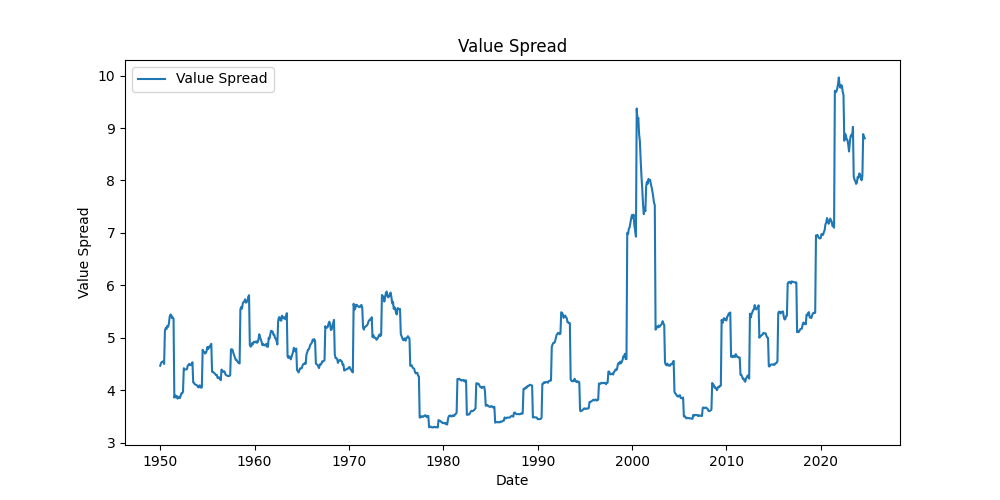
\includegraphics[width=0.8\textwidth]{../figs/Value Spread.png}
    \caption{The value spread timeseries 1950 - 2024}
    \label{fig:value_spread}
\end{figure}


  \section{Measurement of Market Efficiency}
\label{sec:market_efficiency}

In this section, we will introduce the $Beta\_SSE$ estimate, which is our proposed measure of market inefficiency based on the unbiasedness regressions framework.

\subsection{Unbiasedness Regressions}

\noindent The unbiasedness regression is a simple OLS regression of the cumulative logarithmic return of the asset over a normalized window of time $\mathrm{SP500}_{[0, T]}$, on a subset of the
logarithmic cumulative returns, $\mathrm{SP500}_{[0, t]}$, where $t \leq T$, and $t$ is the number of months from the beginning of the window.
 \footnote{$\mathrm{SP500}_{[0, 1]}$ is the matrix of returns of the SP500 from January 1950 to February 1950, February 1950 to March 1950, \dots, August 2024 to September 2024, September 2024 to October 2024.\newline
$\mathrm{SP500}_{[0, 2]}$ would be the matrix of cumulative returns from January 1950 to March 1950, February 1950 to April 1950, \dots August 2024 to October 2024, and so on for the entire dataset.}

\begin{equation}
    \begin{aligned}
        \mathrm{SP500}_{[0, T]} &= \alpha_t + \beta_t \mathrm{SP500}_{[0, t]} + \epsilon_{t}, \hfill \text{   where } 0 \leq t \leq T.
    \end{aligned}
\end{equation}

\noindent For an illustrative example, let $T = 36$, so that the window $[0, T]$ represents a 3-year period, and let us look at the returns of the SP500.

\noindent For $t=1$, the regression is of the form:
\begin{equation}
    \mathrm{SP500}_{[0, 36]} = \alpha + \beta \mathrm{SP500}_{[0, 1]} + \epsilon
\end{equation}

\noindent From this regression we extract the coefficient $\beta$ and the $R^2$ value.
The regression is repeated for $t=2, t=3, ..., t=36$, and the coefficients $\beta$ are plotted against $t$, the depth of the cumulative return window.
We plot the $\beta$ coefficients against $t$ to get a sense of the market's ability to process information over time (Figure~\ref{fig:sp_500_unbiasedness}).

\begin{figure}[h!]
    \centering
    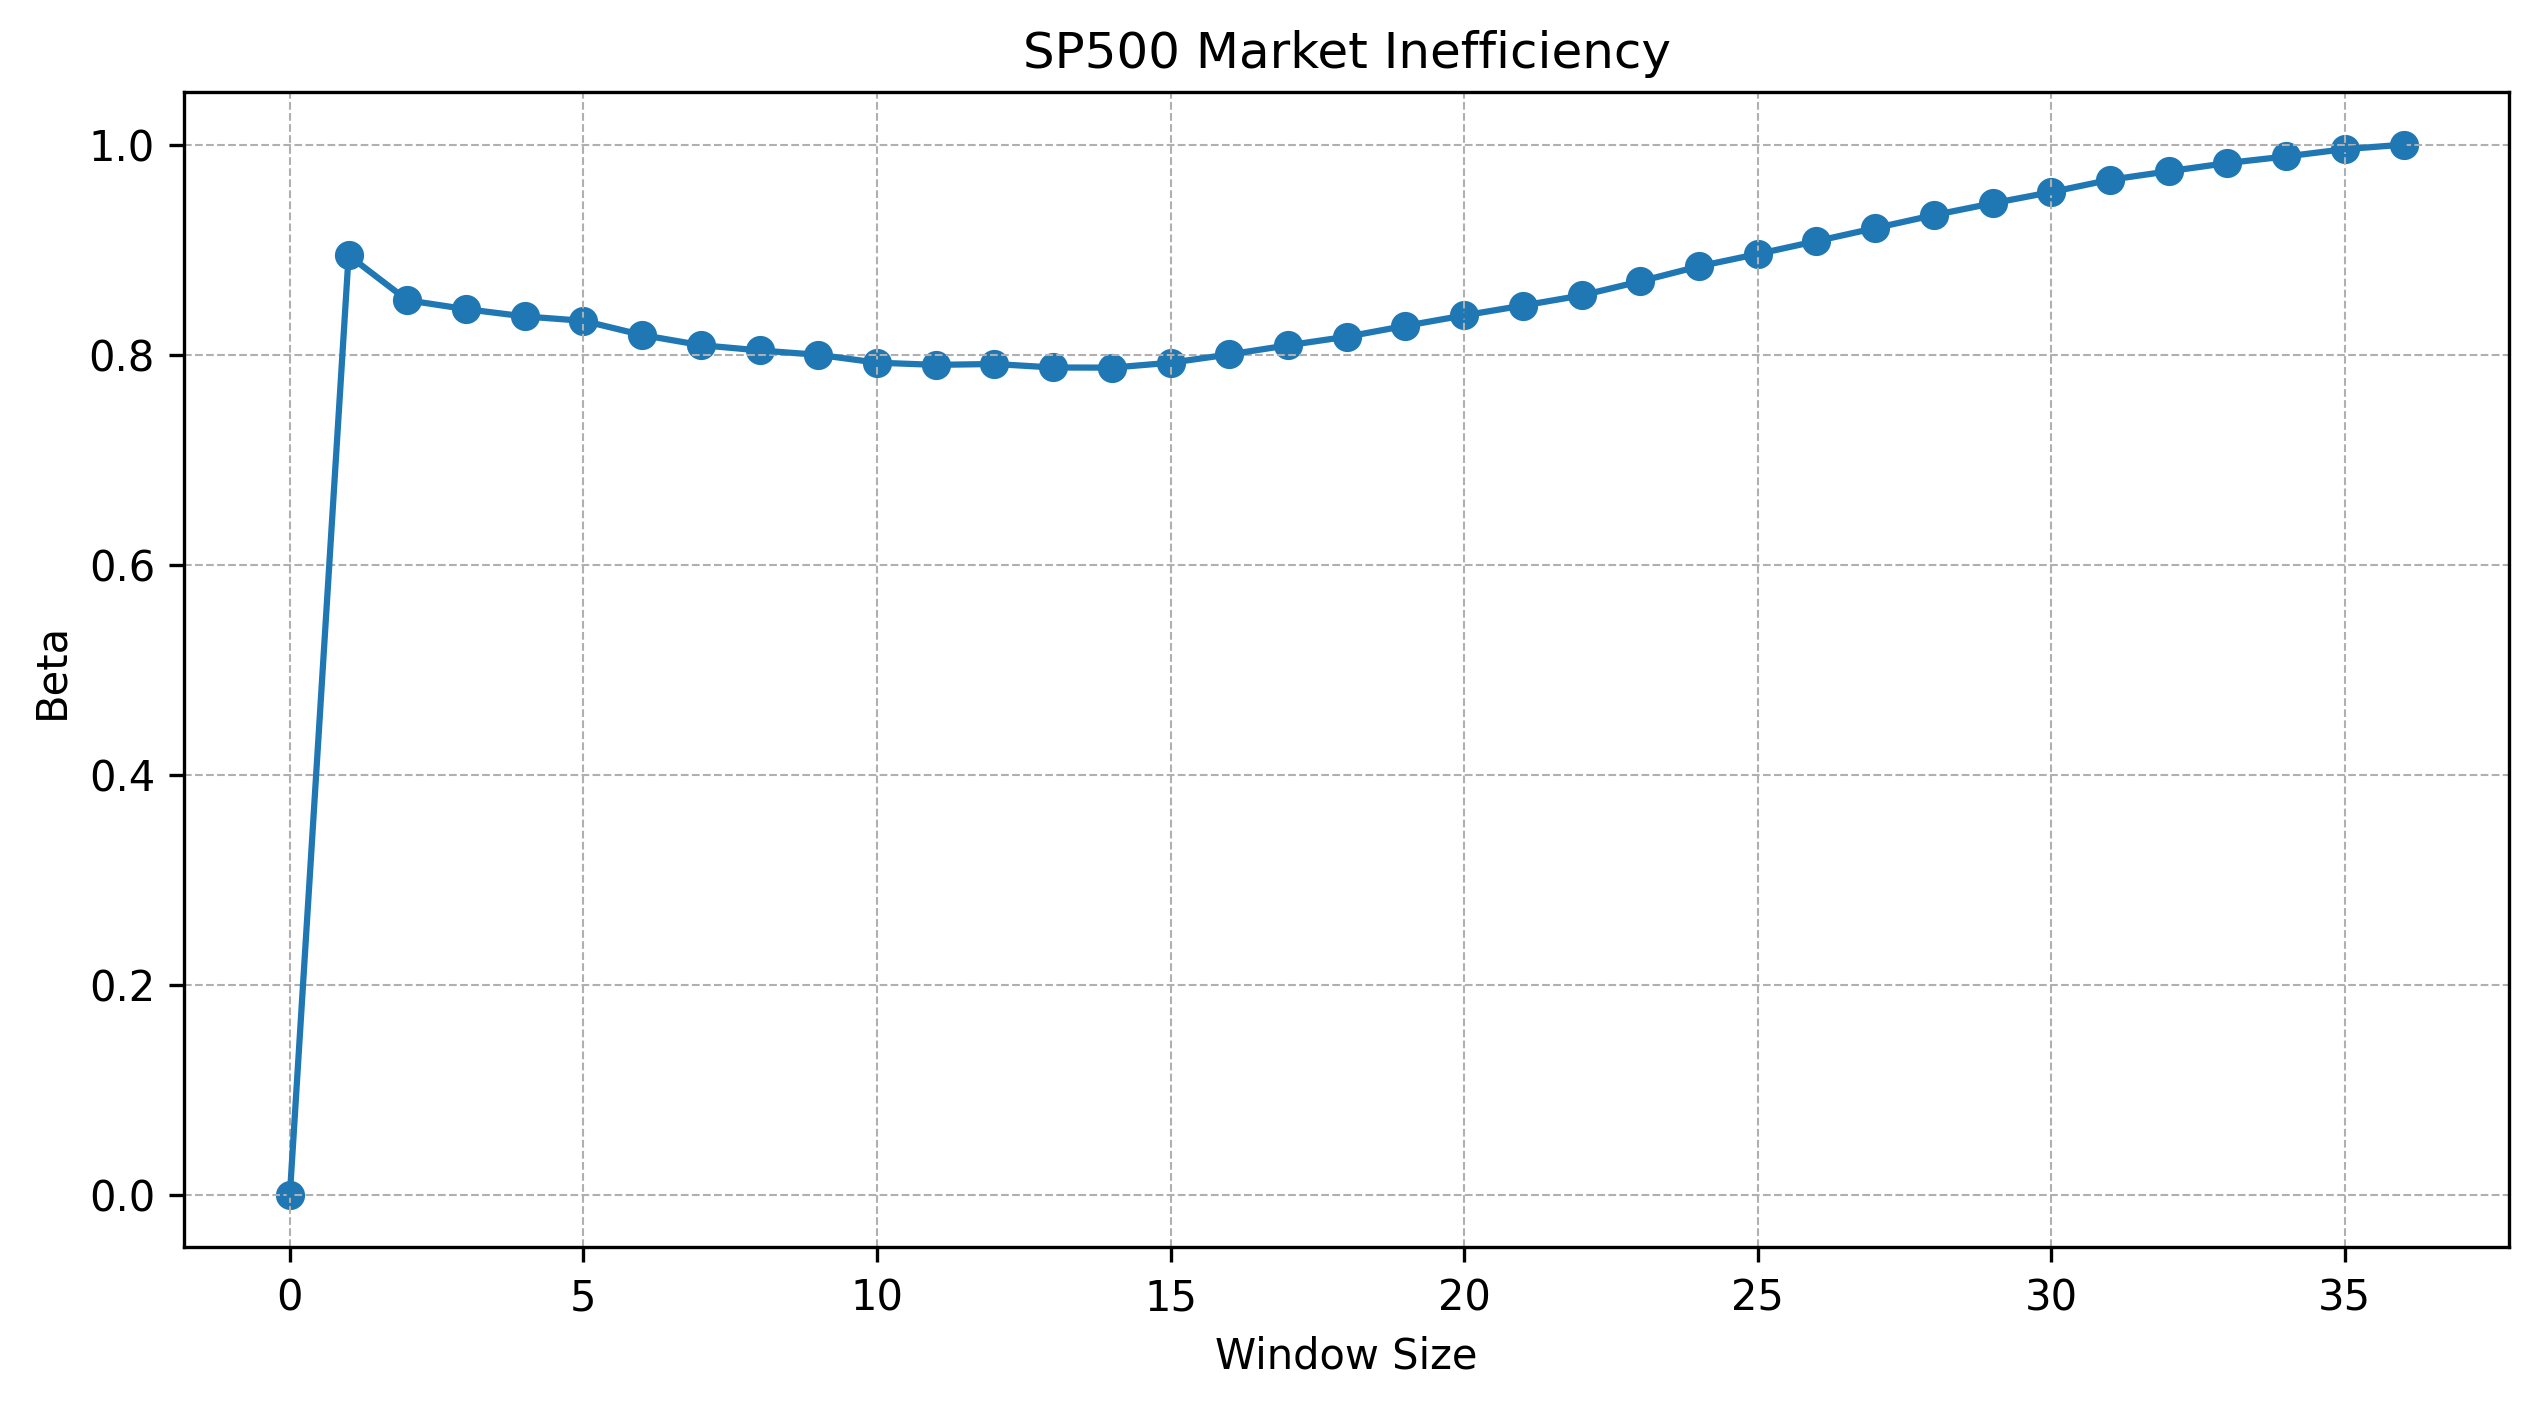
\includegraphics[width=1\textwidth]{../figs/SP500 Market Inefficiency.png}
    \caption{An unbiasedness regression on the SP500 (1950 - 2024) showing the market's tendancy to overreact.}
    \label{fig:sp_500_unbiasedness}
\end{figure}

$\beta_t = 1$ for all $t$ when log prices move efficiently, following a random walk. When 
$\beta_t = 1$ the partial returns from $0$ to $t$ provide a forecast of the return from $t$ to $T$ \citep{mincer_zarnowitz_1969}
 that is as efficient as possible and does not need to be amplified or dampened. 
 If $\beta_t < 1$, the partial return is dampened in the total returns, therefore there was a temporary component in prices which decays representing an “overreaction” \citep{barclay_hendershott_2003}.
Conversely, if $\beta_t > 1$, the partial return is amplified in the total return, suggesting the market had improperly processed the information relevant in pricing the T sized window, and has underreacted.

In this paper we will be focusing on the $\beta_t$ coefficient, but an explanation of the $R^2$ is provided in the Appendix for completeness and intuition building. 
We now have the foundation to construct a score for market efficiency.

\subsection{$Beta\_SSE$ Score}

\begin{figure}[h!]
    \centering
    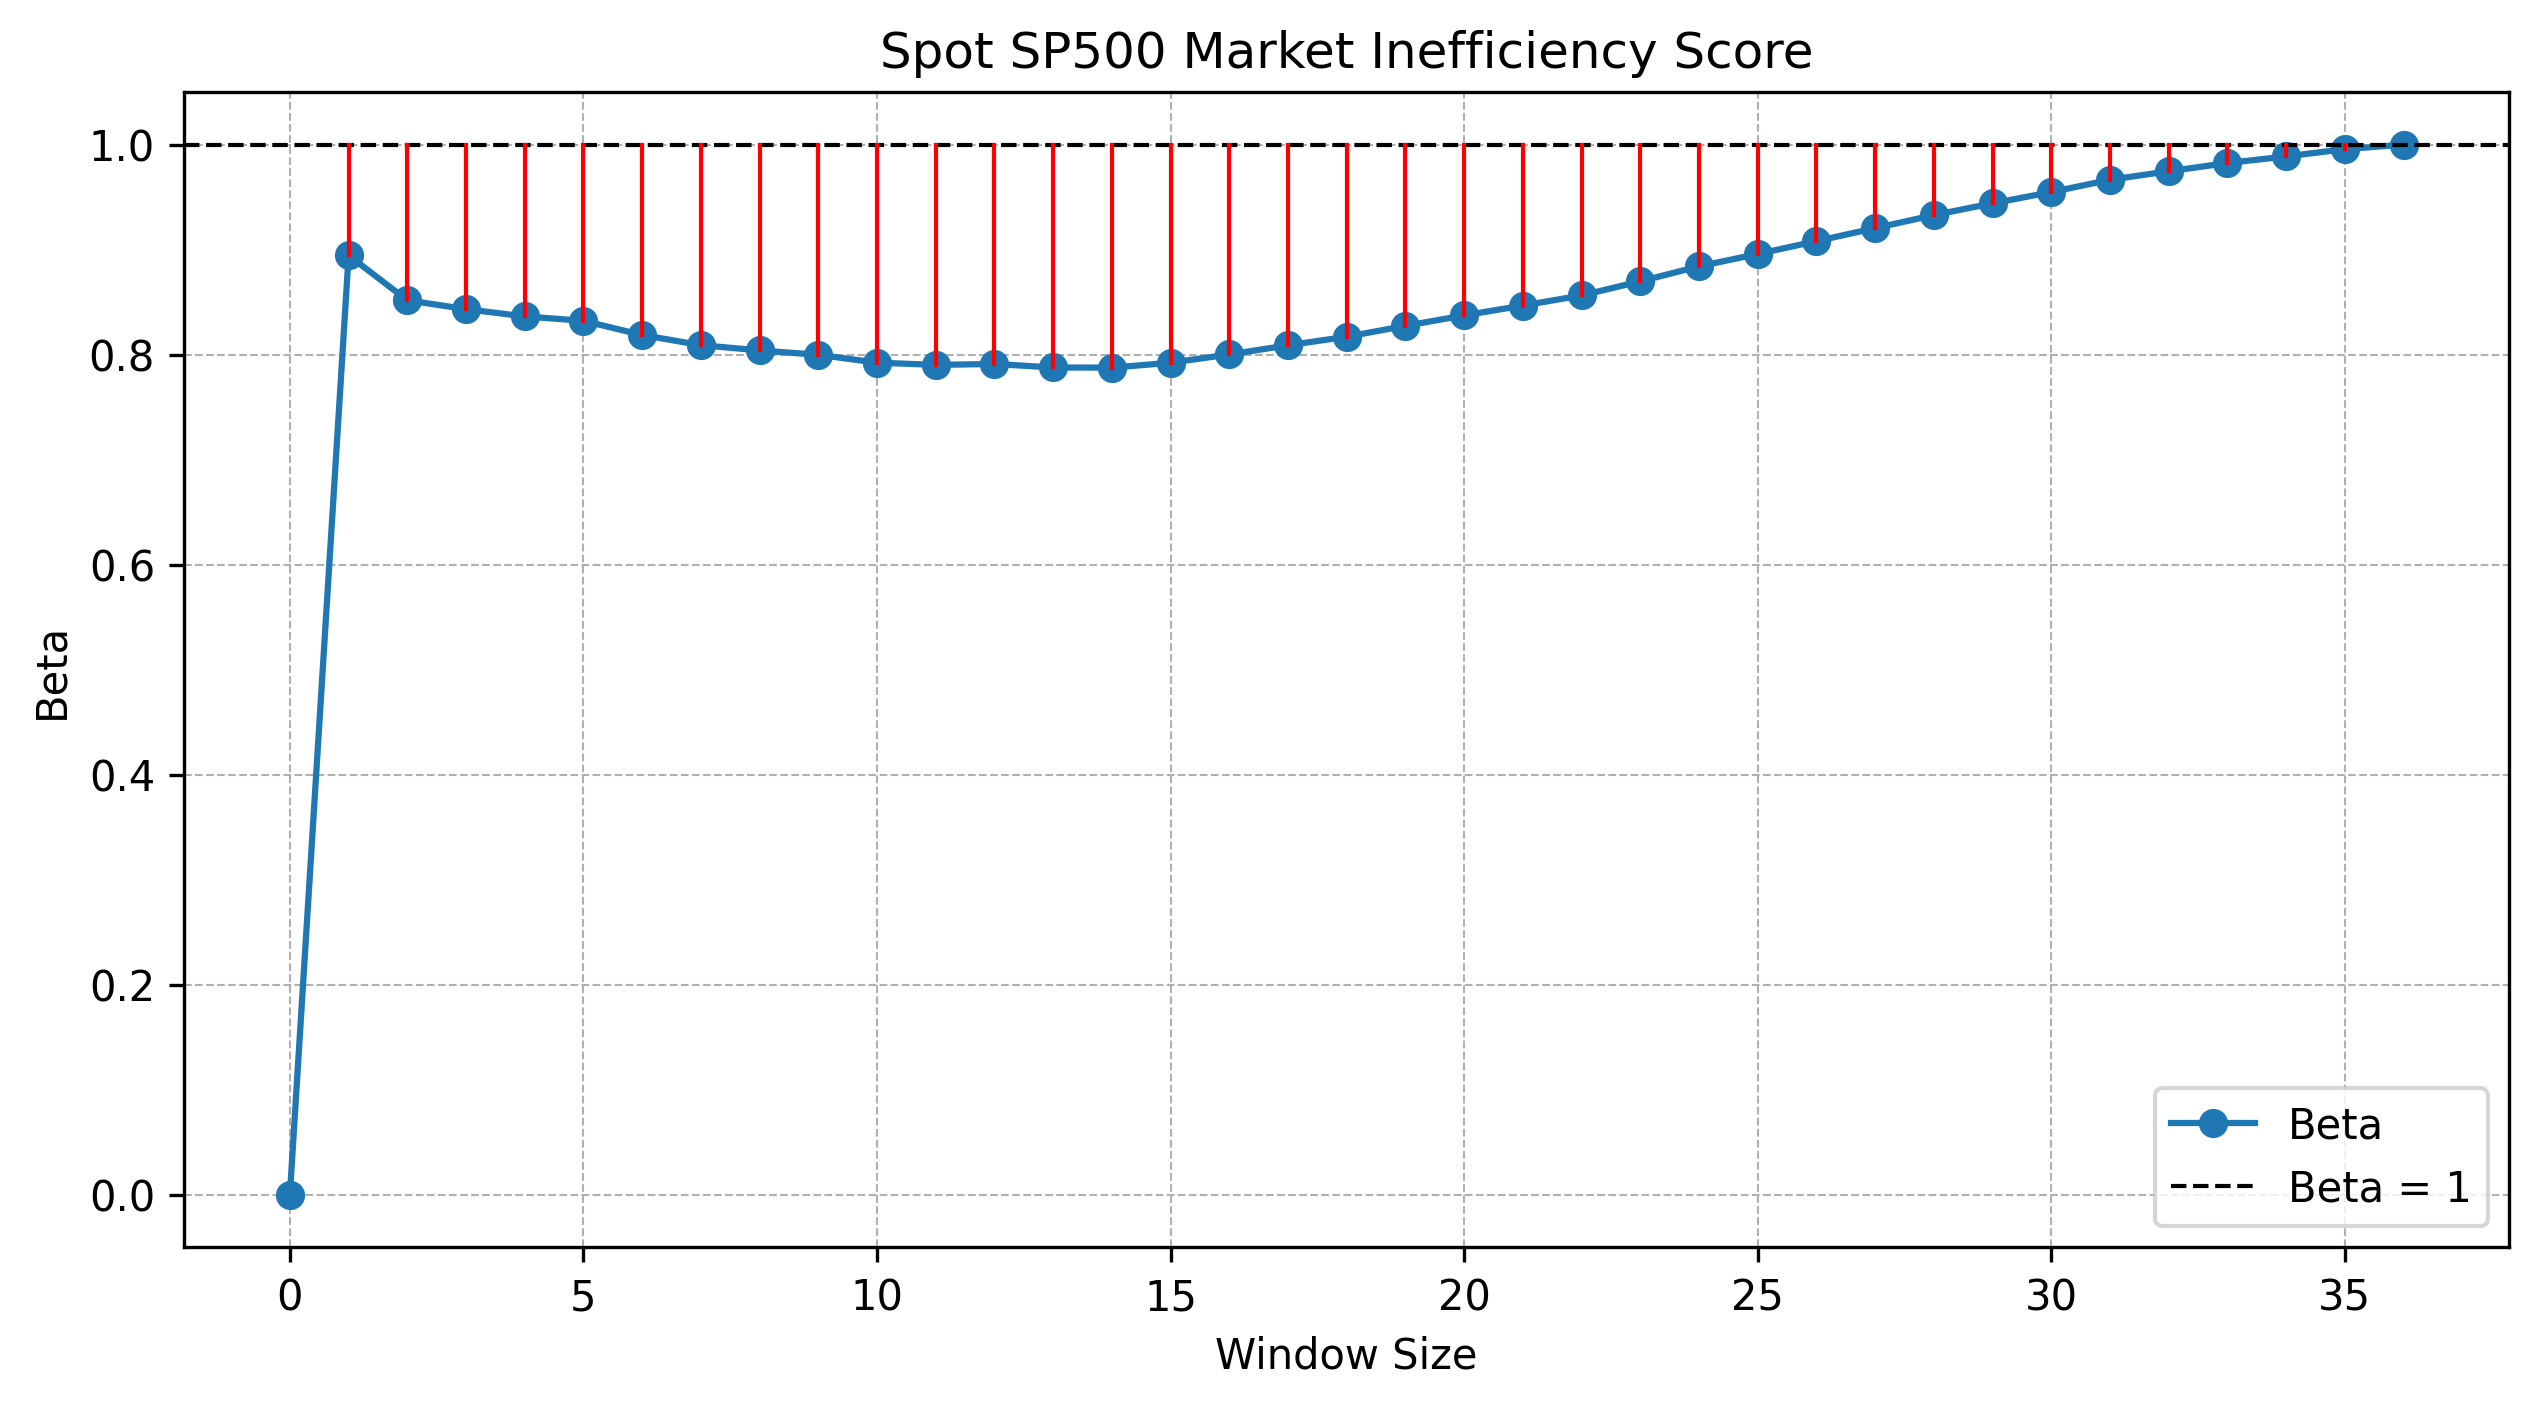
\includegraphics[width=1\textwidth]{../figs/Spot SP500 Market Inefficiency Score.png}
    \caption{The $Beta\_SSE$ score visualization for the SP500 (1950 - 2024). The $Beta\_SSE$ score is a measure of market efficiency at a point in time, and is the sum of 
    the squares of the red distances. To construct a timeseries of the $Beta\_SSE$ score, we run this regression for shingled five-year windows and plot their sums.}
    \label{fig:sp_500_unbiasedness_sse}
\end{figure}

We have established the unbiasedness regression infrastructure, and that a $\beta_t < 1$ indicates overreaction, a $\beta_t > 1$ indicates underreaction, and $\beta_t = 1$ indicates efficiency.
To construct a score that measures the level of market inefficiency at a point in time, we have to create a spot representation of the $\beta_t$ graph for a time period.

We define the $Beta\_SSE$ score as the sum of the squared differences between $\beta_t$ and the horizontal line at $\beta = 1$, for all $t$ in the window.
Since a $\beta_t = 1$ indicates efficiency, the $Beta\_SSE$ score will be lower when the market is more efficient and larger when the market is less efficient, whether by under- or over-reaction.
We provide a visual representation of the $Beta\_SSE$ score for the S\&P500 over our entire data window in Figure~\ref{fig:sp_500_unbiasedness_sse}.

% To construct a time series of these scores, we run the unbiasedness regressions on a rolling window of five years.
To construct a time series of these scores, we split our entire period of S\&P500 returns in shingled 5-year windows. Each window is 5 years long, and the window is moved forward by 1 month at a time.
We run the same sequence of unbiasedness regressions as we did for the entire period in Figure~\ref{fig:sp_500_unbiasedness}, however on each window independently, and calculate the $Beta\_SSE$ score for each window.
So $Beta\_SSE_t$ is constructed from the unbiasedness regressions on windows of the SP500 returns from $t-60$ to $t$.
 Note that our unbiasedness regressions extend out to $t+36$, so $Beta\_SSE_t$ score isn't tradable at time $t$ but at time $t+36$.
\footnote{Consider the rolling window [January 2000, January 2005], the observation starting at January 2005 ($t=0$ on January 2005) requires the window of returns from January 2005 to January 2008 to make $\mathrm{SP500}_{[0, 36]}$.}
This is by design, a measure of market inefficiency at a time $t$ is to be representative of the market's ability to price the $T$ months ahead.

$Beta\_SSE_t$ is calculated as follows:

\begin{equation}
    \begin{aligned}
        Beta\_SSE_t &= \sum_{i=0}^{36} (\beta_{t,i} - 1)^2
    \end{aligned}
\end{equation}

Where $\beta_{t,i}$ is the $\beta$ coefficient from the unbiasedness regression from a 
window starting on the date $t$, at the $i$th depth of the unbiasedness window.

  
  \section{Results}
\label{sec:results}

Using the $Beta\_SSE$ score, we construct a time series of the level of market efficiency as seen in Figure~\ref{fig:sp_500_SSE_beta_ts}.
\begin{figure}[h!]
    \centering
    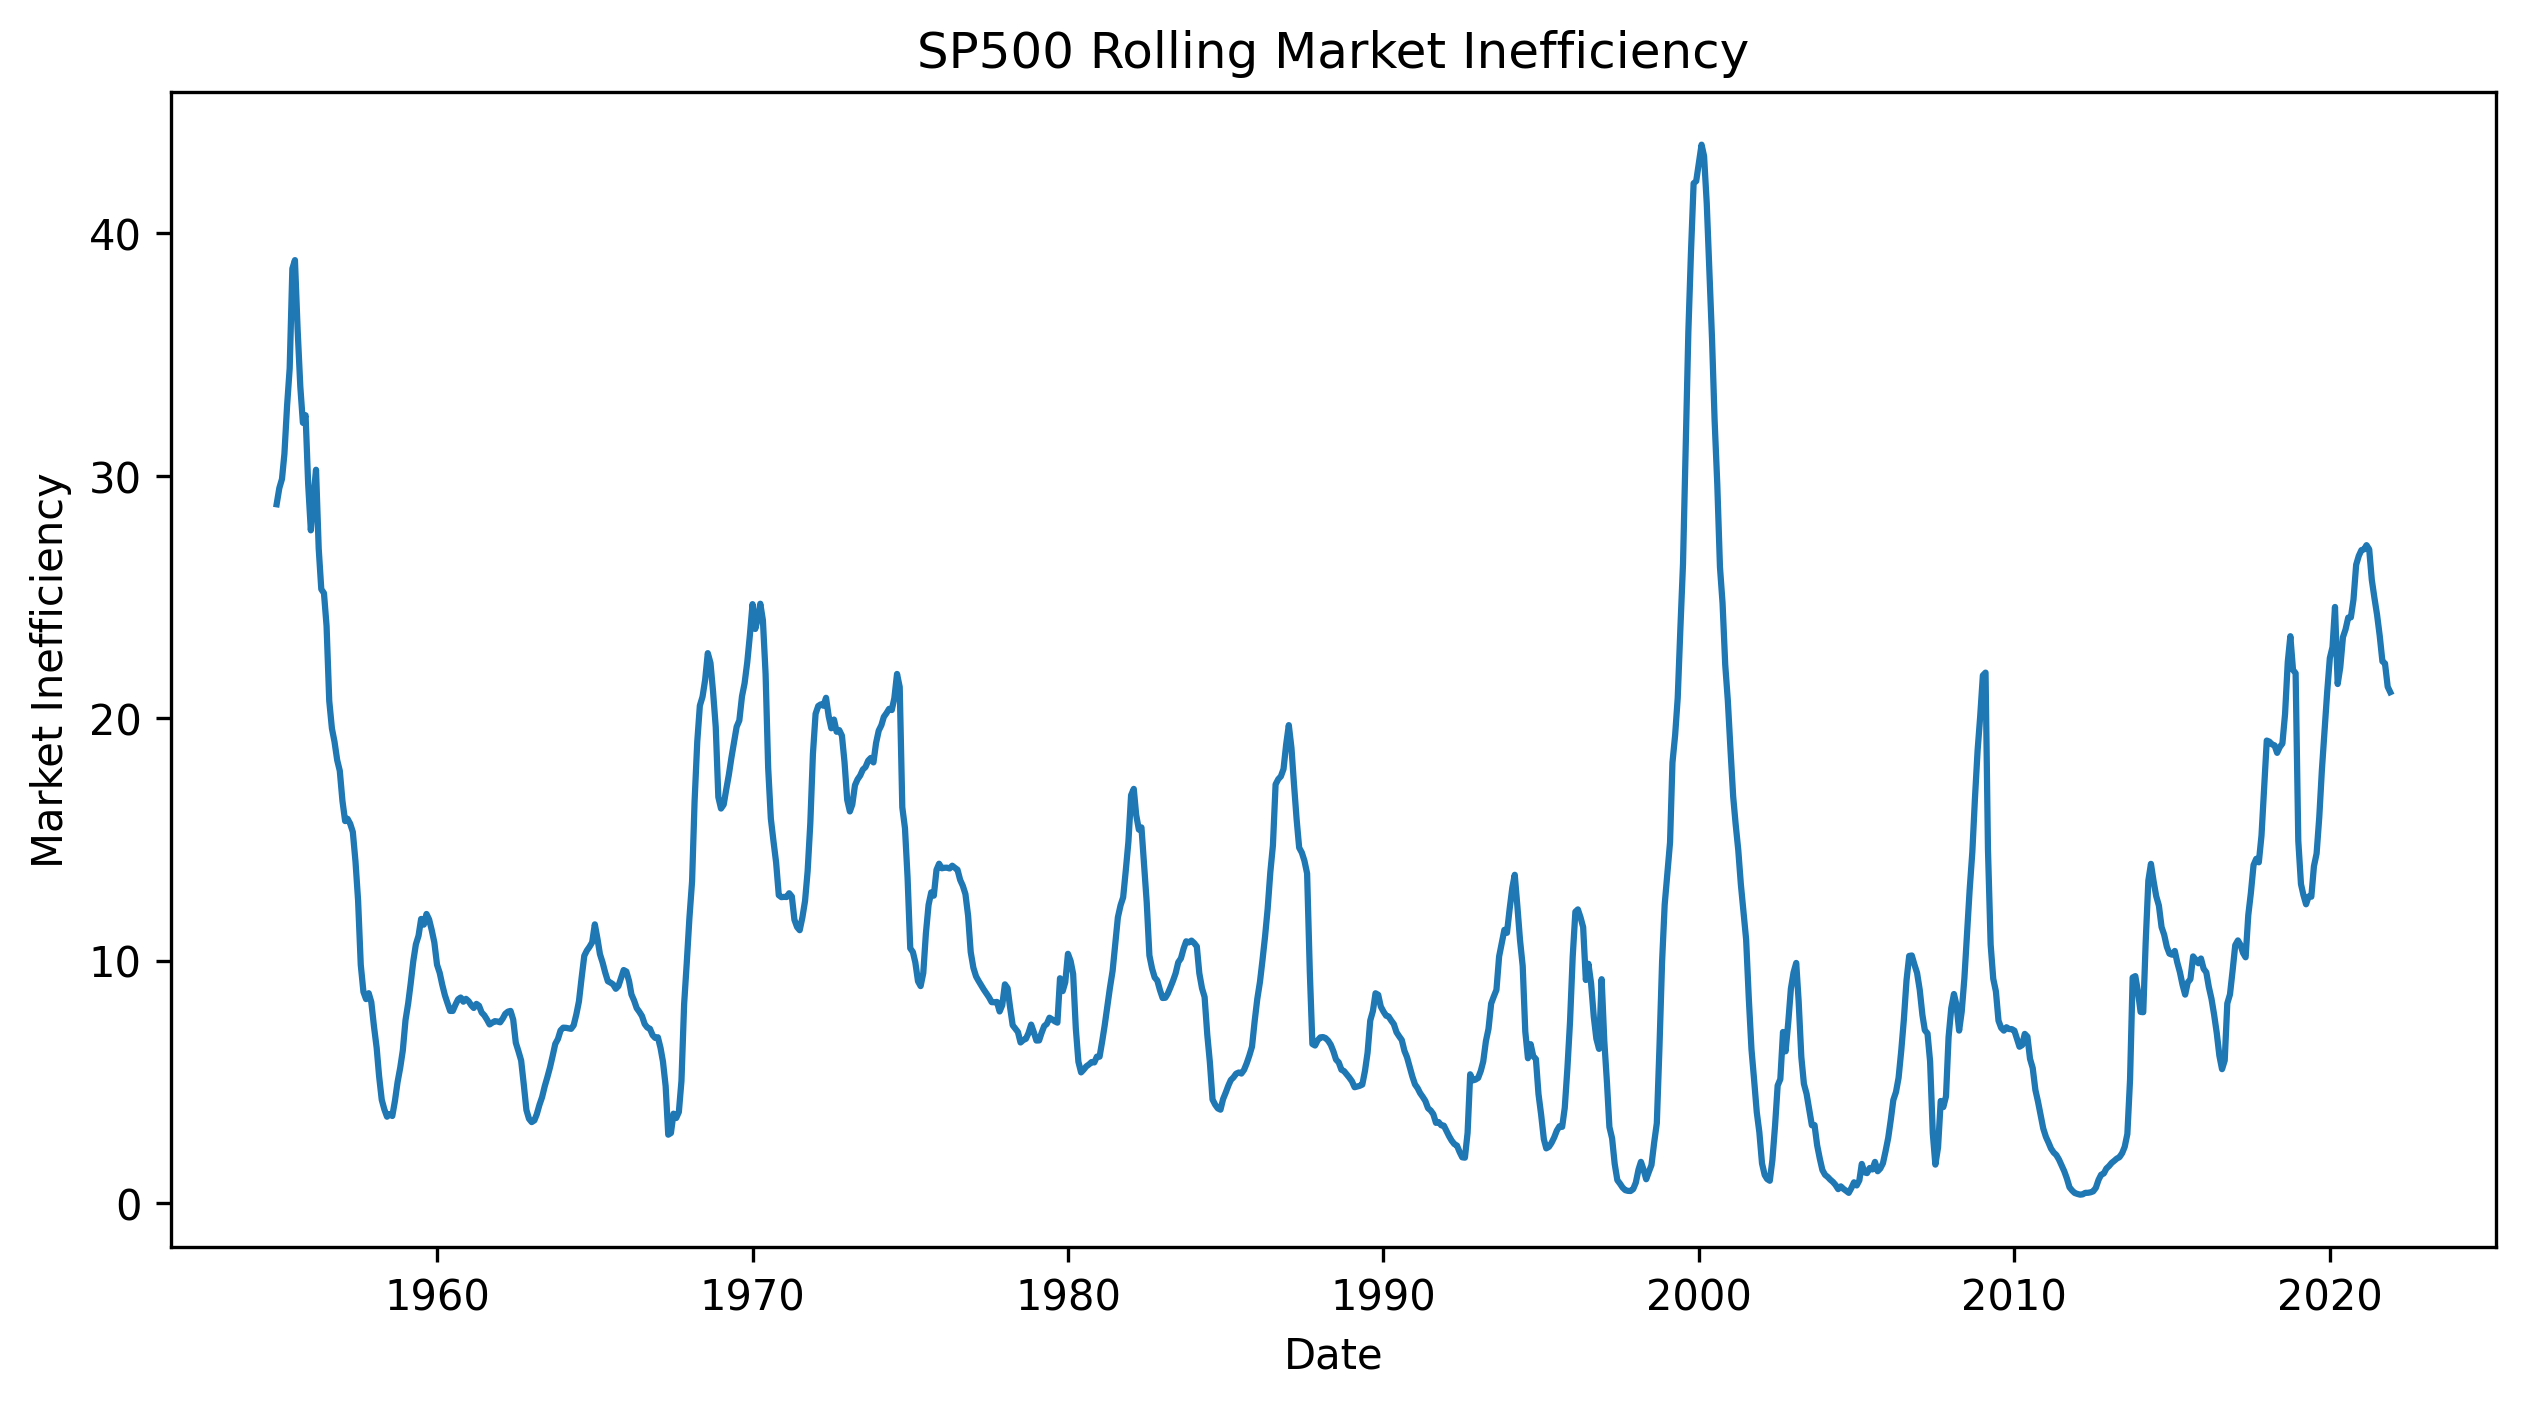
\includegraphics[width=1\textwidth]{../figs/SP500 Rolling Market Inefficiency.png}
    \caption{The $Beta\_SSE$ score time series of the SP500 (1950 - 2024) showing mean reversion and periods of inefficiency.}
    \label{fig:sp_500_SSE_beta_ts}
\end{figure}

We see the market is inefficient around the dot-com bubble, the 2008 financial crisis, and the COVID-19 pandemic, which is in line with our expectations.
We can visually assess that the market is not uniformly efficient. Instead, it goes through periods of higher inefficiency followed by reversion to efficiency.
We also see that the market has been increasingly inefficient in the last decade, which is in line with \citet{asness_2024}.

Empirically we can test the mean reversion through an Augmented Dickey-Fuller test \citep{cheung1995lag} on the $Beta\_SSE$ time series, which is significant at the 0.1\% level.

Figure~\ref{value_spread_beta_sse} shows the value spread and the $Beta\_SSE$ score time series. We see visually that the two are cointegrated, which we test with
the Engle-Granger two-step cointegration test, which is significant at the 0.1\% level.

\begin{figure}[h!]
    \centering
    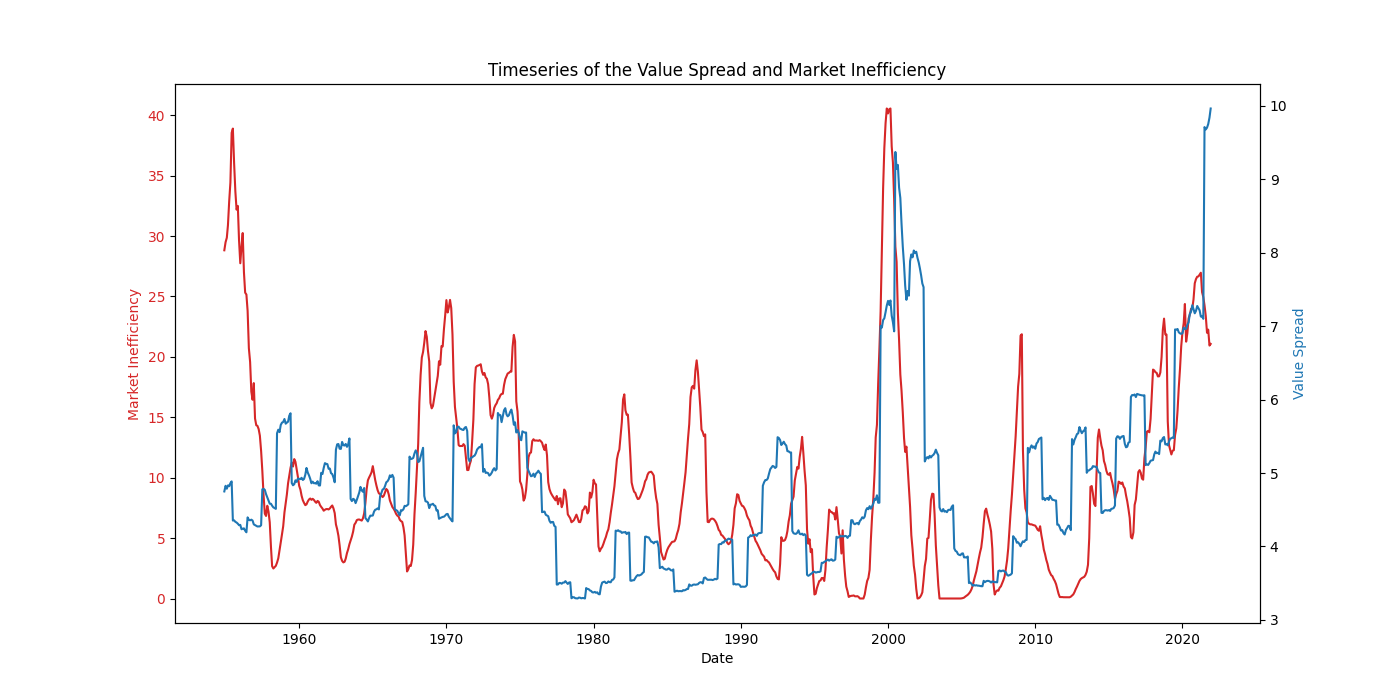
\includegraphics[width=1\textwidth]{../figs/Value Spread and Market Inefficiency.png}
    \caption{The value spread, and market inefficiency move together, and have been increasing in tandem for the last decade.}
    \label{value_spread_beta_sse}
\end{figure}


  \section{Discussion}
\label{sec:conclusion}
\subsection{Summary}
In this paper we construct a measure of market efficiency using \citet{fama_EMH}'s definition of informational efficiency. Our measure is based on unbiasedness
regressions, and captures where the market has inefficient expectations. We build on \citet{asness_2024}'s case on inefficient
value spreads by showing a high correlation of market inefficiency and value spreads in the last decade.

\subsection{Drifting Inefficiency}
We learn the market's ability to present value future prices has weakened over the last decade. The cause of which is worth investigating
in future work. Either the market has been fundamentally more inefficient due to some microstructure, or the world could be in a regime of such innovation and technological change that the market has been systematically forced to revise its
present values of future expectations with accelerating error. This may not be entirely far-fetched, the last decade has seen the rise of the internet,
the proliferation of smartphones, and the rise of machine learning. These are all innovations that have changed the way we live and work, learn and build.
It is obvious the rate of innovation is accelerating, but is the market correctly pricing the higher moment, the rate of innovation acceleration?
Perhaps the markets haven't reached the level of sophistication to correctly price the current accelerating rate of innovation, indicating that
the rate of innovation is a systematic surprise and the cause of $Beta_/SSE$ drift. 

\subsection{Limitations and Future Work}
A limitation of this paper is that we have not established causality between market inefficiency and value spreads. This is a topic for future work.
They are clearly correlated in the last decade, but we cannot say that one causes the other. It is possible that 
growth stocks' high expectations are reasonable, value spreads are reflecting this new regime of expectations, and our co-moving inefficiency
is because of the unprecedented (Therefore difficult to price) nature of these innovations. \citet{asness_2024} argues otherwise, showing possible explanations and dismissing them, but he caveats that this
is not a complete proof. An implication of their co-movement is on portfolio management, if value spreads do widen during periods of inefficiency, portfolio managers with risk-premia mandates may choose to underweigh their value exposure during inefficient regimes, and lever back up once 
markets tend back to efficiency. Conversely, anomalies such as momentum should outperform during periods of informational inefficiency as the 
market comes to grips with unexpected information flows.

In future work we hope to investigate the decomposition of market inefficiency into under-reaction and over-reaction components.
There is an existing literature on the market's tendency to overreact and the robustness of our methodology would be strengthened if it aligns with
the current state of the literature. Additionally, since our measure has a forward-looking bias, attempting to forecast $Beta\_SSE$ would make it 
more practical for its use in portfolio and risk management.

  \newpage
  \bibliographystyle{chicago}
  \bibliography{references}

  \newpage
  \section*{Appendix}
  \renewcommand{\thesection}{\Alph{section}}
  \setcounter{section}{0}
  \section{Appendix}
\label{sec:appendix}

\subsection{Unbiasedness Regressions}
In this Appendix we build on the intuition behind the unbiasedness regressions.

\end{document}